\documentclass[border=5mm]{standalone}
\usepackage[utf8]{inputenc}
\usepackage[T1]{fontenc}
\usepackage{amsmath}
\usepackage{tikz}
\usepackage{pgfplots}
\pgfplotsset{compat=1.18}
\usetikzlibrary{arrows.meta}
\definecolor{utnblue}{RGB}{0, 51, 102}

% Ej11a: h(t) = e^{-2t}u(t)  <-->  g(t) = (1/2)(1-e^{-2t})u(t)

\begin{document}
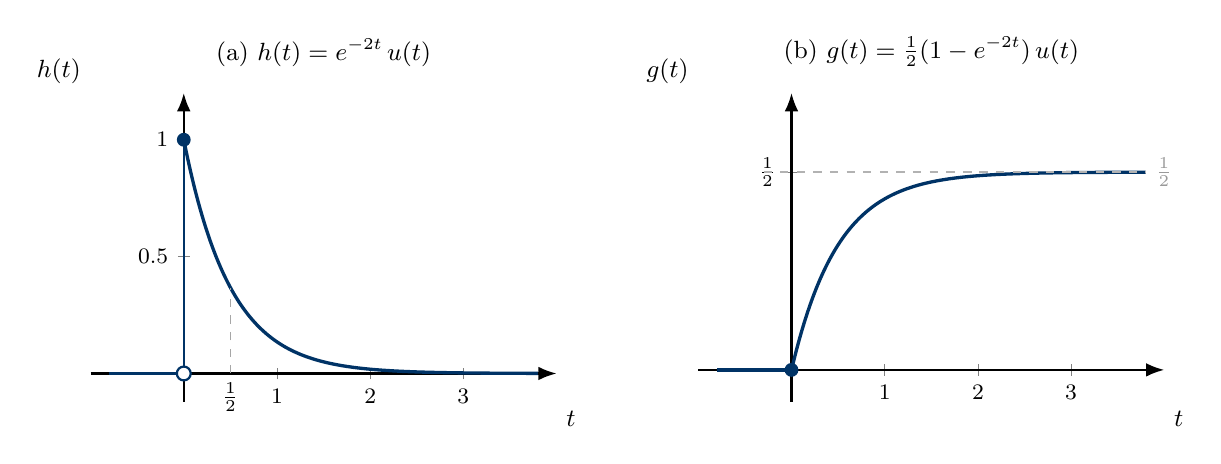
\begin{tikzpicture}[>=Latex, font=\small]

% ---- Panel (a): h(t) = e^{-2t}u(t) ----
\begin{axis}[
    name=ax1,
    width=7.5cm, height=5.5cm,
    axis lines=center,
    xlabel={$t$},
    ylabel={$h(t)$},
    xlabel style={anchor=north west, at={(axis description cs:1,0)}},
    ylabel style={font=\small, rotate=0, anchor=south east, at={(axis description cs:0,1)}},
    xmin=-1, xmax=4,
    ymin=-0.12, ymax=1.2,
    clip=false,
    axis line style={->, thick},
    xtick={0,1,2,3},
    ytick={0,0.5,1},
    every tick label/.style={font=\footnotesize},
    title={\small (a) $h(t)=e^{-2t}\,u(t)$},
]
    % zero for t<0
    \addplot[domain=-0.8:0, samples=2, very thick, utnblue] {0};
    % e^{-2t} for t>=0
    \addplot[domain=0:3.8, samples=200, very thick, utnblue] {exp(-2*x)};
    % vertical jump at t=0
    \draw[utnblue, thick] (axis cs:0,0) -- (axis cs:0,1);
    \fill[utnblue] (axis cs:0,1) circle (2.5pt);
    \fill[white]   (axis cs:0,0) circle (2.5pt);
    \draw[utnblue, thick] (axis cs:0,0) circle (2.5pt);
    % tau_0 guide
    \draw[dashed, gray!70, thin] (axis cs:0.5, 0) -- (axis cs:0.5, {exp(-1)});
    \node[font=\footnotesize, below] at (axis cs:0.5, 0) {$\frac{1}{2}$};
\end{axis}

% ---- Panel (b): g(t) = (1/2)(1 - e^{-2t})u(t) ----
\begin{axis}[
    name=ax2,
    at={(ax1.east)}, anchor=west, xshift=1.8cm,
    width=7.5cm, height=5.5cm,
    axis lines=center,
    xlabel={$t$},
    ylabel={$g(t)$},
    xlabel style={anchor=north west, at={(axis description cs:1,0)}},
    ylabel style={font=\small, rotate=0, anchor=south east, at={(axis description cs:0,1)}},
    xmin=-1, xmax=4,
    ymin=-0.08, ymax=0.7,
    clip=false,
    axis line style={->, thick},
    xtick={0,1,2,3},
    ytick={0,0.5},
    yticklabels={$0$, $\frac{1}{2}$},
    every tick label/.style={font=\footnotesize},
    title={\small (b) $g(t)=\frac{1}{2}(1-e^{-2t})\,u(t)$},
]
    % zero for t<0
    \addplot[domain=-0.8:0, samples=2, very thick, utnblue] {0};
    % (1/2)(1-e^{-2t}) for t>=0
    \addplot[domain=0:3.8, samples=200, very thick, utnblue] {0.5*(1 - exp(-2*x))};
    % asymptote at 1/2
    \addplot[domain=-0.3:3.8, dashed, thick, gray!60] {0.5};
    \node[font=\footnotesize, gray!80, right] at (axis cs:3.8, 0.5) {$\frac{1}{2}$};
    % dot at origin
    \fill[utnblue] (axis cs:0, 0) circle (2.5pt);
\end{axis}

\end{tikzpicture}
\end{document}
